\documentclass[11pt]{article}
\usepackage[letterpaper,margin=0.85in,top=1.05in,headheight=14pt]{geometry}
\usepackage{amsmath,amssymb}
\usepackage{enumitem}
\usepackage{fancyhdr}
\usepackage{multicol}
\usepackage{tikz}

\pagestyle{fancy}
\fancyhf{}
\fancyhead[L]{\small Honors Algebra 1 Readiness}
\fancyhead[R]{\small Name: \underline{\hspace{1.8in}}}
\fancyfoot[C]{\small \thepage}
\renewcommand{\headrulewidth}{0.4pt}

\setlist[enumerate]{itemsep=0pt, topsep=4pt, parsep=0pt, leftmargin=*}

\begin{document}

\section*{Part A: Negative Numbers and Order of Operations}
\noindent\textit{Evaluate each expression completely. Show each major order-of-operations step.}
\begin{multicols}{2}
\begin{enumerate}
  \item $10 + (-14)$
  \vspace{1.1cm}
  \item $-3 + (-14)$
  \vspace{1.1cm}
  \item $11 \cdot (-7)$
  \vspace{1.1cm}
  \item $8 \cdot (-2)$
  \vspace{1.1cm}
  \item $-3 + (-12) \cdot 5$
  \vspace{1.1cm}
  \item $-7 + (-9) \cdot (-10)$
  \vspace{1.1cm}
  \item $2^{2} - 17 \cdot 6$
  \vspace{1.1cm}
  \item $9^{3} - (-4) \cdot 7$
  \vspace{1.1cm}
  \item $17 - 10 \cdot (7 + 17)$
  \vspace{1.1cm}
  \item $(3 + 23)^{2} \div 4$
  \vspace{1.1cm}
\end{enumerate}
\end{multicols}

\section*{Part B: Ratios, Proportions, and Percentages}
\noindent\textit{Solve each problem. Show your setup and simplify your answer.}
\begin{multicols}{2}
\begin{enumerate}
  \item $\dfrac{7}{14} = \dfrac{x}{42}$
  \vspace{1.4cm}
  \item $\dfrac{x}{11} = \dfrac{12}{44}$
  \vspace{1.4cm}
  \item $\dfrac{x}{14} = \dfrac{72}{112}$
  \vspace{1.4cm}
  \item $30\%$ of $72$
  \vspace{1.4cm}
  \item $15\%$ of $300$
  \vspace{1.4cm}
  \item $60\%$ of $600$
  \vspace{1.4cm}
  \item from $50$ to $60$
  \vspace{1.4cm}
  \item from $5$ to $3$
  \vspace{1.4cm}
  \item Liam pays $\$9$ for $3$ pencils. Find the price per pencil.
  \vspace{1.4cm}
  \item Kai pays $\$20$ for $4$ bagels. Find the price per bagel.
  \vspace{1.4cm}
\end{enumerate}
\end{multicols}

\section*{Part C: Exponents, Roots, and Scientific Notation}
\noindent\textit{Simplify or evaluate completely. Write powers with positive exponents.}
\begin{multicols}{2}
\begin{enumerate}
  \item $8x^{8} \cdot 3x^{9}$
  \vspace{1.2cm}
  \item $2x^{2} \cdot 7x^{6}$
  \vspace{1.2cm}
  \item $\dfrac{9x^{12}}{x^{6}}$
  \vspace{1.2cm}
  \item $\dfrac{6x^{11}}{x^{3}}$
  \vspace{1.2cm}
  \item $(5x^{4})^{4}$
  \vspace{1.2cm}
  \item $(9x^{2})^{4}$
  \vspace{1.2cm}
  \item $\sqrt{49}$
  \vspace{1.2cm}
  \item $\sqrt[3]{64}$
  \vspace{1.2cm}
  \item $9400$
  \vspace{1.2cm}
  \item $(4.565 \times 10^{4}) \div (8.3 \times 10^{2})$
  \vspace{1.2cm}
\end{enumerate}
\end{multicols}

\section*{Part D: Simplifying and Factoring Expressions}
\noindent\textit{Simplify or factor as directed. Show distribution and like-term steps.}
\begin{multicols}{2}
\begin{enumerate}
  \item $2x + 7 + 10x + 12$
  \vspace{1.3cm}
  \item $-x + 3 + 2x + 5$
  \vspace{1.3cm}
  \item $3x - 2 - 8x + 5$
  \vspace{1.3cm}
  \item $-5x + x^{2} - 8x - 12x^{2}$
  \vspace{1.3cm}
  \item $2x^{2} - 11x^{2} + 11x - 2x$
  \vspace{1.3cm}
  \item $10x^{2} - 6x + 10x + 3x^{2}$
  \vspace{1.3cm}
  \item $12(2x - 4) + 12x + 10$
  \vspace{1.3cm}
  \item $11(3x - 8) + 4x - 1$
  \vspace{1.3cm}
  \item $\operatorname{GCF}\left(60x^{3}, 84x^{1}\right)$
  \vspace{1.3cm}
  \item $\operatorname{GCF}\left(24x^{1}, 9x^{2}\right)$
  \vspace{1.3cm}
\end{enumerate}
\end{multicols}

\section*{Part E: Solving Linear Equations}
\noindent\textit{Solve each equation for $x$. Show your steps and check when practical.}
\begin{multicols}{2}
\begin{enumerate}
  \item $10x + 12 = 17$
  \vspace{1.9cm}
  \item $4x + 8 = 32$
  \vspace{1.9cm}
  \item $9(x + 9) - 12 = -3$
  \vspace{1.9cm}
  \item $2(4x - 6) + 6 = -94$
  \vspace{1.9cm}
  \item $7x - 7 = 6x + 1$
  \vspace{1.9cm}
  \item $-7x + 8 = 7x + 78$
  \vspace{1.9cm}
  \item $-\dfrac{8}{5}x + 10 = \dfrac{138}{25}$
  \vspace{1.9cm}
  \item $\dfrac{x}{3} - 14 = -\dfrac{22}{3}$
  \vspace{1.9cm}
  \item $\dfrac{-3}{x} = \dfrac{7}{6}$
  \vspace{1.9cm}
  \item $\dfrac{-3}{x} = \dfrac{4}{3}$
  \vspace{1.9cm}
\end{enumerate}
\end{multicols}

\section*{Part F: Linear Inequalities}
\noindent\textit{Solve each inequality for $x$. Reverse the inequality when required.}
\begin{multicols}{2}
\begin{enumerate}
  \item $x - 1 \le -12$
  \vspace{1.7cm}
  \item $x - 12 < 8$
  \vspace{1.7cm}
  \item $11x - 3 \ge -14$
  \vspace{1.7cm}
  \item $-4x + 1 > -19$
  \vspace{1.7cm}
  \item $-12x - 11 \le -8x - 43$
  \vspace{1.7cm}
  \item $10x - 5 > -11x + 247$
  \vspace{1.7cm}
  \item $-\dfrac{7}{2}x + 17 \ge 52$
  \vspace{1.7cm}
  \item $-\dfrac{9}{4}x - 13 \le -\dfrac{43}{4}$
  \vspace{1.7cm}
  \item $-72 \le -8x - 8 < 0$
  \vspace{1.7cm}
  \item $-68 < -7x + 9 < 65$
  \vspace{1.7cm}
\end{enumerate}
\end{multicols}

\section*{Part G: Coordinate Plane and Linear Relationships}
\noindent\textit{Find the requested slope, line equation, or distance.}
\begin{multicols}{2}
\begin{enumerate}
  \item $y = 7x + 6$
  \vspace{1.7cm}
  \item $y = 9x - 7$
  \vspace{1.7cm}
  \item $(-6, -32)$ and $(8, 31)$
  \vspace{1.7cm}
  \item $(4, 4)$ and $(6, 7)$
  \vspace{1.7cm}
  \item $(-5, -21)$ and $(-1, -1)$
  \vspace{1.7cm}
  \item $(-9, -39)$ and $(-2, -11)$
  \vspace{1.7cm}
  \item $(-3, 14)$ and $(-9, 22)$
  \vspace{1.7cm}
  \item $(-4, -7)$ and $(4, -22)$
  \vspace{1.7cm}
  \item $m = 9$ through $(-8, -67)$
  \vspace{1.7cm}
  \item $m = 6$ through $(-4, -32)$
  \vspace{1.7cm}
\end{enumerate}
\end{multicols}

\section*{Part H: Functions and Patterns}
\noindent\textit{Evaluate, analyze, or find the requested rule or term.}
\begin{multicols}{2}
\begin{enumerate}
  \item $f(x) = x^{2} + 6x + 4, \quad f(-3)$
  \vspace{1.5cm}
  \item $f(x) = 2x^{2} - 2x - 9, \quad f(3)$
  \vspace{1.5cm}
  \item $f(x) = 3x^{2} - 6x + 7, \quad f(4)$
  \vspace{1.5cm}
  \item $f(x) = 6x^{2} - 2x + 9, \quad f(1)$
  \vspace{1.5cm}
  \item $\{(-8, -4), (3, -8), (10, 5), (7, 8), (-2, -10)\}$
  \vspace{1.5cm}
  \item $\{(0, 9), (5, -2), (-1, -9), (-4, -10), (-10, 7)\}$
  \vspace{1.5cm}
  \item $\{(7, 1), (-6, -2), (-10, 2), (9, 2), (2, 6)\}$
  \vspace{1.5cm}
  \item $r = 7cs$, solve for $s$
  \vspace{1.5cm}
  \item $6r + 5a = q$, solve for $a$
  \vspace{1.5cm}
  \item $5b + 3u = a$, solve for $u$
  \vspace{1.5cm}
\end{enumerate}
\end{multicols}

\section*{Part I: Geometry Applications}
\noindent\textit{Find the requested measure. Include units when given.}
\begin{enumerate}
  \item All measurements are in in.
\begin{center}
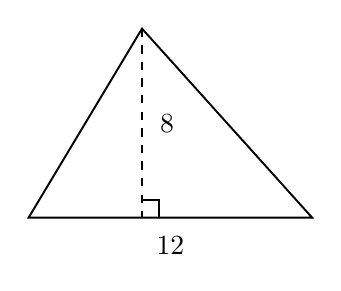
\begin{tikzpicture}[line width=0.7pt]
\draw (0,0) -- (3.600,0) -- (1.440,2.400) -- cycle;
\draw[dashed] (1.440,2.400) -- (1.440,0);
\draw (1.440,0.000) ++(0.220,0) -- ++(0,0.220) -- ++(-0.220,0);
\node at (1.800,-0.350) {$12$};
\node[anchor=west] at (1.540,1.200) {$8$};
\end{tikzpicture}
\end{center}

  \vspace{1.5cm}
  \item All measurements are in in.
\begin{center}
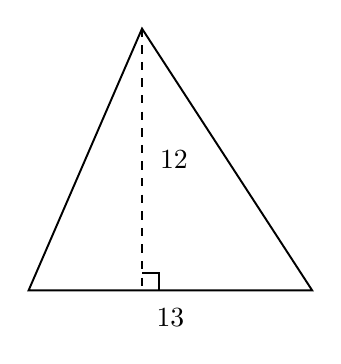
\begin{tikzpicture}[line width=0.7pt]
\draw (0,0) -- (3.600,0) -- (1.440,3.323) -- cycle;
\draw[dashed] (1.440,3.323) -- (1.440,0);
\draw (1.440,0.000) ++(0.220,0) -- ++(0,0.220) -- ++(-0.220,0);
\node at (1.800,-0.350) {$13$};
\node[anchor=west] at (1.540,1.662) {$12$};
\end{tikzpicture}
\end{center}

  \vspace{1.5cm}
  \item All measurements are in cm.
\begin{center}
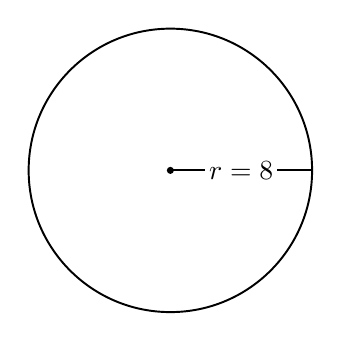
\begin{tikzpicture}[line width=0.7pt]
\draw (0,0) circle (1.800);
\draw (0,0) -- (1.800,0);
\fill (0,0) circle (0.045);
\node[fill=white, inner sep=1.5pt] at (0.900,0) {$r = 8$};
\end{tikzpicture}
\end{center}

  \vspace{1.5cm}
  \item All measurements are in ft.
\begin{center}
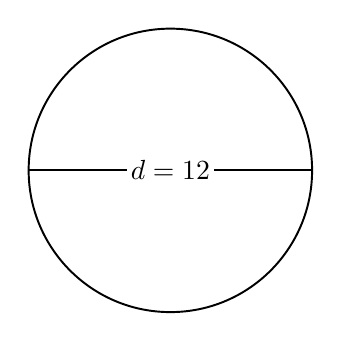
\begin{tikzpicture}[line width=0.7pt]
\draw (0,0) circle (1.800);
\draw (-1.800,0) -- (1.800,0);
\fill (0,0) circle (0.045);
\node[fill=white, inner sep=1.5pt] at (0,0) {$d = 12$};
\end{tikzpicture}
\end{center}

  \vspace{1.5cm}
  \item A right triangle. All measurements are in ft.
\begin{center}
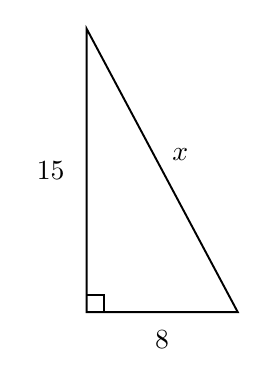
\begin{tikzpicture}[line width=0.7pt]
\draw (0,0) -- (1.920,0) -- (0,3.600) -- cycle;
\draw (0.000,0.000) ++(0.220,0) -- ++(0,0.220) -- ++(-0.220,0);
\node at (0.960,-0.350) {$8$};
\node[anchor=east] at (-0.150,1.800) {$15$};
\node[anchor=south west] at (0.960,1.800) {$x$};
\end{tikzpicture}
\end{center}

  \vspace{1.5cm}
  \item A right triangle. All measurements are in cm.
\begin{center}
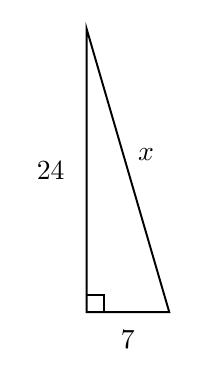
\begin{tikzpicture}[line width=0.7pt]
\draw (0,0) -- (1.050,0) -- (0,3.600) -- cycle;
\draw (0.000,0.000) ++(0.220,0) -- ++(0,0.220) -- ++(-0.220,0);
\node at (0.525,-0.350) {$7$};
\node[anchor=east] at (-0.150,1.800) {$24$};
\node[anchor=south west] at (0.525,1.800) {$x$};
\end{tikzpicture}
\end{center}

  \vspace{1.5cm}
  \item A right triangle. All measurements are in units.
\begin{center}
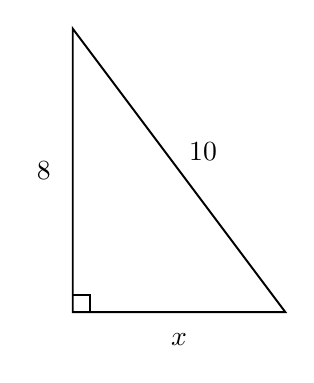
\begin{tikzpicture}[line width=0.7pt]
\draw (0,0) -- (2.700,0) -- (0,3.600) -- cycle;
\draw (0.000,0.000) ++(0.220,0) -- ++(0,0.220) -- ++(-0.220,0);
\node at (1.350,-0.350) {$x$};
\node[anchor=east] at (-0.150,1.800) {$8$};
\node[anchor=south west] at (1.350,1.800) {$10$};
\end{tikzpicture}
\end{center}

  \vspace{1.5cm}
  \item A right triangle. All measurements are in in.
\begin{center}
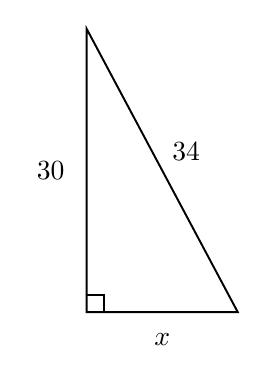
\begin{tikzpicture}[line width=0.7pt]
\draw (0,0) -- (1.920,0) -- (0,3.600) -- cycle;
\draw (0.000,0.000) ++(0.220,0) -- ++(0,0.220) -- ++(-0.220,0);
\node at (0.960,-0.350) {$x$};
\node[anchor=east] at (-0.150,1.800) {$30$};
\node[anchor=south west] at (0.960,1.800) {$34$};
\end{tikzpicture}
\end{center}

  \vspace{1.5cm}
  \item A rectangular prism. All measurements are in ft.
\begin{center}
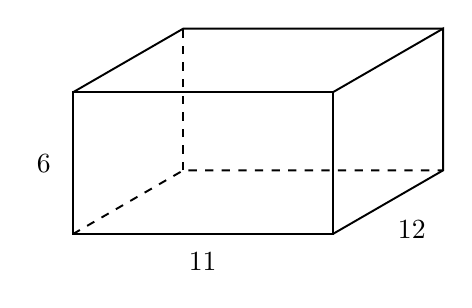
\begin{tikzpicture}[line width=0.7pt]
\draw (0.000,0.000) -- (3.300,0.000) -- (3.300,1.800) -- (0.000,1.800) -- cycle;
\draw (3.300,0.000) -- (4.703,0.810) -- (4.703,2.610) -- (3.300,1.800);
\draw (0.000,1.800) -- (1.403,2.610) -- (4.703,2.610);
\draw[dashed] (0.000,0.000) -- (1.403,0.810) -- (4.703,0.810);
\draw[dashed] (1.403,0.810) -- (1.403,2.610);
\node at (1.650,-0.350) {$11$};
\node[anchor=north west] at (4.001,0.305) {$12$};
\node[anchor=east] at (-0.150,0.900) {$6$};
\end{tikzpicture}
\end{center}

  \vspace{1.5cm}
  \item A rectangular prism. All measurements are in m.
\begin{center}
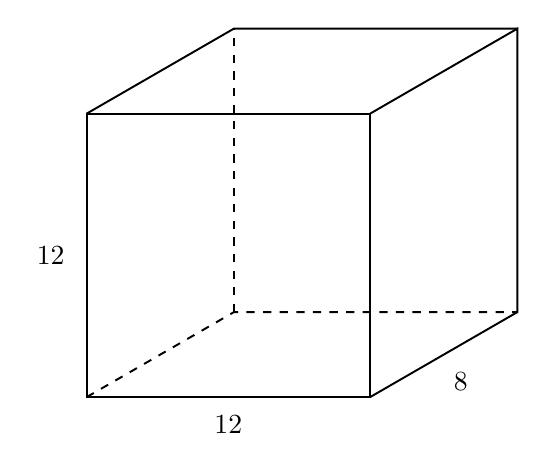
\begin{tikzpicture}[line width=0.7pt]
\draw (0.000,0.000) -- (3.600,0.000) -- (3.600,3.600) -- (0.000,3.600) -- cycle;
\draw (3.600,0.000) -- (5.471,1.080) -- (5.471,4.680) -- (3.600,3.600);
\draw (0.000,3.600) -- (1.871,4.680) -- (5.471,4.680);
\draw[dashed] (0.000,0.000) -- (1.871,1.080) -- (5.471,1.080);
\draw[dashed] (1.871,1.080) -- (1.871,4.680);
\node at (1.800,-0.350) {$12$};
\node[anchor=north west] at (4.535,0.440) {$8$};
\node[anchor=east] at (-0.150,1.800) {$12$};
\end{tikzpicture}
\end{center}

  \vspace{1.5cm}
\end{enumerate}

\section*{Part J: Word Problems and Modeling}
\noindent\textit{Define a variable, write a model, solve, and interpret the answer.}
\begin{enumerate}
  \item Wes buys $8$ marbles each week and already owns $21$ marbles. After how many weeks will Wes have $117$ marbles?
  \vspace{2.0cm}
  \item Noah buys $6$ tickets each week and already owns $13$ tickets. After how many weeks will Noah have $43$ tickets?
  \vspace{2.0cm}
  \item Sam buys $5$ stickers each week and already owns $2$ stickers. After how many weeks will Sam have $62$ stickers?
  \vspace{2.0cm}
  \item Priya rides at a steady $11$ miles per hour and travels $66$ miles. How many hours does the ride take?
  \vspace{2.0cm}
  \item Ethan rides at a steady $11$ miles per hour and travels $33$ miles. How many hours does the ride take?
  \vspace{2.0cm}
  \item Jonas rides at a steady $19$ miles per hour and travels $95$ miles. How many hours does the ride take?
  \vspace{2.0cm}
  \item A sticker originally costs $\$80$. Maya uses a $25\%$ off coupon. How many dollars does Maya save?
  \vspace{2.0cm}
  \item A marble originally costs $\$40$. Jonas uses a $40\%$ off coupon. How many dollars does Jonas save?
  \vspace{2.0cm}
  \item Plan A charges $\$50$ plus $\$17$ per month. Plan B charges $\$5$ plus $\$22$ per month. After how many months do the two plans cost the same?
  \vspace{2.0cm}
  \item Plan A charges $\$49$ plus $\$9$ per month. Plan B charges $\$22$ plus $\$12$ per month. After how many months do the two plans cost the same?
  \vspace{2.0cm}
\end{enumerate}

\newpage
\fancyhead[L]{\small Honors Algebra 1 Readiness --- Teacher Key}
\section*{Answer Key}
\subsection*{Part A: Negative Numbers and Order of Operations}
\begin{multicols}{3}
\begin{enumerate}
  \item $-4$
  \item $-17$
  \item $-77$
  \item $-16$
  \item $-63$
  \item $83$
  \item $-98$
  \item $757$
  \item $-223$
  \item $169$
\end{enumerate}
\end{multicols}
\subsection*{Part B: Ratios, Proportions, and Percentages}
\begin{multicols}{3}
\begin{enumerate}
  \item $x = 21$
  \item $x = 3$
  \item $x = 9$
  \item $\frac{108}{5}$
  \item $45$
  \item $360$
  \item $20\%$
  \item $-40\%$
  \item $\$3$ per pencil
  \item $\$5$ per bagel
\end{enumerate}
\end{multicols}
\subsection*{Part C: Exponents, Roots, and Scientific Notation}
\begin{multicols}{3}
\begin{enumerate}
  \item $24 x^{17}$
  \item $14 x^{8}$
  \item $9 x^{6}$
  \item $6 x^{8}$
  \item $625 x^{16}$
  \item $6561 x^{8}$
  \item $7$
  \item $4$
  \item $9.4 \times 10^{3}$
  \item $5.5 \times 10^{1}$
\end{enumerate}
\end{multicols}
\subsection*{Part D: Simplifying and Factoring Expressions}
\begin{multicols}{3}
\begin{enumerate}
  \item $12 x + 19$
  \item $x + 8$
  \item $3 - 5 x$
  \item $- 11 x^{2} - 13 x$
  \item $- 9 x^{2} + 9 x$
  \item $13 x^{2} + 4 x$
  \item $36 x - 38$
  \item $37 x - 89$
  \item $12 x$
  \item $3 x$
\end{enumerate}
\end{multicols}
\subsection*{Part E: Solving Linear Equations}
\begin{multicols}{3}
\begin{enumerate}
  \item $x = \frac{1}{2}$
  \item $x = 6$
  \item $x = -8$
  \item $x = -11$
  \item $x = 8$
  \item $x = -5$
  \item $x = \frac{14}{5}$
  \item $x = 20$
  \item $x = - \frac{18}{7}$
  \item $x = - \frac{9}{4}$
\end{enumerate}
\end{multicols}
\subsection*{Part F: Linear Inequalities}
\begin{multicols}{3}
\begin{enumerate}
  \item $x \le -11$
  \item $x < 20$
  \item $x \ge -1$
  \item $x < 5$
  \item $x \ge 8$
  \item $x > 12$
  \item $x \le -10$
  \item $x \ge -1$
  \item $-1 < x \le 8$
  \item $-8 < x < 11$
\end{enumerate}
\end{multicols}
\subsection*{Part G: Coordinate Plane and Linear Relationships}
\begin{multicols}{3}
\begin{enumerate}
  \item $m = 7$, \quad $b = 6$
  \item $m = 9$, \quad $b = -7$
  \item $m = \frac{9}{2}$
  \item $m = \frac{3}{2}$
  \item $y = 5x + 4$
  \item $y = 4x - 3$
  \item $10$
  \item $17$
  \item $y = 9x + 5$
  \item $y = 6x - 8$
\end{enumerate}
\end{multicols}
\subsection*{Part H: Functions and Patterns}
\begin{multicols}{3}
\begin{enumerate}
  \item $-5$
  \item $3$
  \item $31$
  \item $13$
  \item domain: $\{-8, -2, 3, 7, 10\}$; range: $\{-10, -8, -4, 5, 8\}$
  \item domain: $\{-10, -4, -1, 0, 5\}$; range: $\{-10, -9, -2, 7, 9\}$
  \item domain: $\{-10, -6, 2, 7, 9\}$; range: $\{-2, 1, 2, 6\}$
  \item $s = \dfrac{r}{7c}$
  \item $a = \dfrac{q - 6r}{5}$
  \item $u = \dfrac{a - 5b}{3}$
\end{enumerate}
\end{multicols}
\subsection*{Part I: Geometry Applications}
\begin{multicols}{3}
\begin{enumerate}
  \item $48$ square in
  \item $78$ square in
  \item $64 \pi$ square cm
  \item $36 \pi$ square ft
  \item $17$ ft
  \item $25$ cm
  \item $6$ units
  \item $16$ in
  \item $792$ cubic ft
  \item $1152$ cubic m
\end{enumerate}
\end{multicols}
\subsection*{Part J: Word Problems and Modeling}
\begin{multicols}{3}
\begin{enumerate}
  \item $12\text{ weeks}$
  \item $5\text{ weeks}$
  \item $12\text{ weeks}$
  \item $6\text{ hours}$
  \item $3\text{ hours}$
  \item $5\text{ hours}$
  \item $20\text{ dollars}$
  \item $16\text{ dollars}$
  \item $9\text{ months}$
  \item $9\text{ months}$
\end{enumerate}
\end{multicols}

\end{document}
